% FRAGMENT A07 (drafter A: class model and main results)
% REPLACES: main.tex lines 386–564 ("\section{3. Competition and information}" to "… determines when information can be sustained in equilibrium.")
%   This covers Sections 3.1, 3.2, and 3.3, including Figure 1.
% ANCHOR FOR ANOTHER FRAGMENT: M1_04 ("INSERT AFTER main.tex line 564") goes at the comment
%   "ANCHOR M1_04" at the end of this fragment.
% LABELS KEPT: sec-payoffs, sec-acquisition-profits-and-target-proceeds, eq:paper-4,
%   eq:paper-5, result-proposition-1, eq:paper-6, fig:1, sec-inference, eq:paper-7,
%   eq:paper-8, eq:paper-9, eq:paper-10, sec-informed-trading-incentives, eq:paper-11.
% LABELS REMOVED: none.  LABELS ADDED: none.
% CHANGED SYMBOLS: Proposition 1's old G_\theta(F) (gross profit) is renamed g_j(F), because
%   G_j is now the class value cdf. e_r(\mu), P_r(\mu) lose the subscript r (general F).
% NEW SYMBOLS: m(\pi), M(\pi) (posterior bounds; m=m(1/2), M=M(1/2) as before),
%   \kappa(\pi)=\min\{m(\pi),1-M(\pi)\} (trading-bound constant).
% NEW CITATIONS: none.  NUM PLACEHOLDERS: none.
% EQUATION TAGS: (4)–(11) keep their numbers. The per-value identity and the split identity
%   are unnumbered displays.
% SOURCES: Q1_N_main.md Claims 1–4, 6–8 and the split identity (N7); Q4_normalization.md
%   Claim 4 (t+g=theta); SYNTHESIS.md A.1 rows 1–4.

\section{3. Competition and information}\label{sec-payoffs}

\subsection{3.1 Acquisition profits and target
proceeds}\label{sec-acquisition-profits-and-target-proceeds}

The auction determines both the return to preparation and the claim that
informed investors trade. Consider a prepared challenger with value
\(\theta\ge p\). If it wins, it pays \(\max\{p,R\}\); if it loses, the
incumbent pays \(\theta\). The target therefore receives
\(\max\{p,\min(R,\theta)\}\), and the challenger keeps
\((\theta-\max\{p,R\})_+\). A prepared challenger with \(\theta<p\)
cannot bid, and the target receives the reserve if the incumbent's value
meets it, exactly as without entry. For every value at or above the
reserve, the two expected amounts add up to the value:

\[
t(\theta)+g(\theta)=\theta,\qquad \theta\ge p.
\]

The second-price rule passes the whole value of an admissible
challenger to the target and the challenger together. An admissible
value also raises proceeds to at least the reserve, so \(t_j\ge t_0\)
for both classes.

In the point-mass benchmark with the uniform incumbent, integrating over
\(R\) gives

\[
\begin{aligned}
t_0&=p\left(1-\frac p r\right),&
t_H&=\frac r2+\frac{p^2}{2r},\\
t_L&=\ell-\frac{\ell^2-p^2}{2r},&
g_H&=h-\frac r2-\frac{p^2}{2r},\\
g_L&=\frac{\ell^2-p^2}{2r},&
\Delta_T(r)&=\frac{(r-\ell)^2}{2r}.
\end{aligned}
\tag{4}\label{eq:paper-4}
\]

The relevant derivatives are

\[
\begin{aligned}
B_r(\mu)&=g_L+\mu(g_H-g_L),\\
\Delta_T'(r)&=\frac12-\frac{\ell^2}{2r^2}>0,\\
g_H'(r)&=-\frac12+\frac{p^2}{2r^2}<0,
\qquad g_L'(r)=-\frac{\ell^2-p^2}{2r^2}<0.
\end{aligned}
\tag{5}\label{eq:paper-5}
\]

Thus a stronger incumbent lowers acquisition profit at every fixed
belief while making target proceeds more sensitive to challenger
quality. \hyperref[result-proposition-1]{Proposition 1} extends this
opposition to every continuous incumbent distribution and every pair of
classes that satisfies the restrictions of
\hyperref[sec-values-preparation-and-the-sale]{Section 2.2}.

\Needspace{8\baselineskip}

\protect\phantomsection\label{result-proposition-1}{\textbf{Proposition
1 (competition and the two returns to information; analytical).}}
\emph{Let the incumbent's value have a continuous distribution \(F\) on
\([0,\bar r]\), extended by unity above \(\bar r\). For any classes
\(G_H,G_L\) with finite means,}

\[
\begin{aligned}
\Delta_T(F)&=pF(p)D(p^-)+\int_p^\infty[1-F(u)]D(u)\,du,\\
g_j(F)&=\int_p^\infty[1-G_j(u)]F(u)\,du,\qquad j\in\{H,L\}.
\end{aligned}
\tag{6}\label{eq:paper-6}
\]

\emph{Let \(\tilde F\le F\) be a continuous first-order stochastic
strengthening of \(F\). (a) For every pair of classes, it weakly
decreases \(g_H\) and \(g_L\), and hence gross acquisition profit at
every fixed belief. (b) Under the restrictions of
\hyperref[sec-values-preparation-and-the-sale]{Section 2.2}, it weakly
increases the target-payoff spread. (c) The spread weakly increases
under every first-order stochastic strengthening of every continuous
\(F\) if and only if \(D(u)\ge0\) for every \(u>p\) and
\(D(p^-)\le0\); when neither class has an atom at \(p\), this condition
is exactly the pair of restrictions of
\hyperref[sec-values-preparation-and-the-sale]{Section 2.2}. The
decrease in \(g_j\) is strict when
\(\int_p^\infty[1-G_j(u)][F(u)-\tilde F(u)]\,du>0\), and the increase
in (b) is strict when \(\int_p^\infty[F(u)-\tilde F(u)]D(u)\,du>0\).}

The proof works one incumbent value at a time. At a value \(R\) that
meets the reserve, the target receives
\(\min\{R,\max\{\theta,p\}\}\). The expected class difference in
proceeds is then \(\int_p^RD(u)\,du\). Read the integrand as slices
\(D(u)\,du\) of the class value gap at each level \(u>p\). The slice at
\(u\) reaches the target when the incumbent outbids the challenger at
that level and pays its bid. It stays with the challenger otherwise.
A stronger incumbent moves slices to the target. The spread rises and
acquisition profit falls. The reserve adds one term. Below the
reserve, only an admissible challenger buys, at \(p\), and the class
difference is \(pD(p^-)\). A stronger incumbent fails the reserve less
often, so that term shrinks. It can outweigh the moved slices when
the low class is more often inadmissible. Equal admissibility removes
it. \hyperref[paper-appendix]{Appendix A} gives the proof.

Adding the two lines of \eqref{eq:paper-6} under equal admissibility
gives

\[
\Delta_T(F)+g_H(F)-g_L(F)
=\mathbb E_H[\max\{\theta,p\}]-\mathbb E_L[\max\{\theta,p\}]
\]

for every incumbent distribution; in the benchmark the right side is
\(h-\ell\) at every \(r\). A stronger incumbent does not change the
value gap between the classes; it moves the gap from the challenger's
profit to target proceeds.

\setcounter{figure}{0}
\begin{figure}[tbp]\centering\begingroup\singlespacing
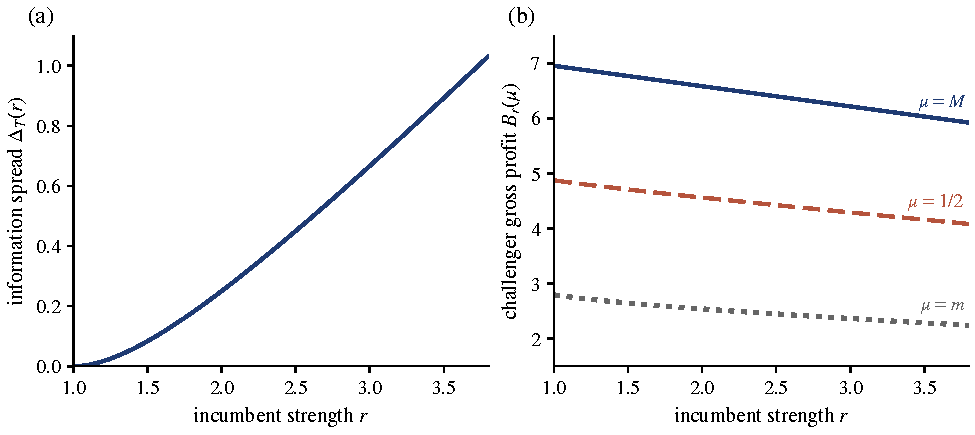
\includegraphics[width=\linewidth]{figures/two_returns.pdf}
\caption{Competition and the two returns to information.}\label{fig:1}
\par\medskip\begin{minipage}{\linewidth}\footnotesize\singlespacing\noindent \textit{Notes.} Panel (a) plots the target-payoff spread \(\Delta_T(r)\); panel (b)
plots gross challenger profit \(B_r(\mu)\) at the posterior bounds
\(m,M\) and the prior \(1/2\). Point-mass benchmark values are \(h=10\),
\(\ell=1\), \(p=0.5\), and \(b=2\), with prior \(1/2\). Values are per target share. These
are acquisition-stage payoffs, before solving trading and entry.\end{minipage}
\endgroup\end{figure}

Figure~\ref{fig:1} shows both effects within the benchmark support. The
target-payoff spread approaches zero as \(r\) approaches \(\ell\), since
the incumbent then almost never outbids a low-value challenger. As \(r\)
increases, the spread rises while gross acquisition profit falls at each
displayed belief. Whether entry rises depends on how this change in
payoffs affects equilibrium information.

\subsection{3.2 What the challenger learns from the
price}\label{sec-inference}

Noise demand bounds the posterior under every feasible trading strategy.
For arbitrary mixed orders, define

\[
\begin{aligned}
a_H(x)&=\int f(x-q)\,d\sigma_H(q),\qquad
&a_L(x)&=\int f(x-q)\,d\sigma_L(q),\\
\mu_X(x)&=\frac{\pi a_H(x)}{\pi a_H(x)+(1-\pi)a_L(x)},\qquad
&m(\pi)&=\frac{\pi}{\pi+(1-\pi)e^{2/b}},\quad
M(\pi)=\frac{\pi}{\pi+(1-\pi)e^{-2/b}}.
\end{aligned}
\tag{7}\label{eq:paper-7}
\]

The posterior satisfies \(m(\pi)\le\mu_X\le M(\pi)\). In the benchmark
\(\pi=1/2\), and I write \(m=m(1/2)=1/(1+e^{2/b})\) and
\(M=M(1/2)=1-m\). For any two orders \(q,q'\in[-1,1]\), the Laplace
density obeys

\[
e^{-2/b}\le\frac{f(x-q)}{f(x-q')}\le e^{2/b}.
\tag{8}\label{eq:paper-8}
\]

Integrating over the conditional order distributions preserves these
inequalities, so \(a_H/a_L\) lies in \([e^{-2/b},e^{2/b}]\). By Bayes'
rule the log odds of \(\mu_X\) are the log odds of \(\pi\) plus
\(\log(a_H/a_L)\), which gives the posterior bounds. Since the price is
a function of flow, the price-based posterior is a conditional
expectation of \(\mu_X\) and has the same bounds. A preparation decision
requiring a belief above \(M(\pi)\) cannot be induced by any equilibrium
price.

A low-cost challenger pays nothing to prepare, and its expected gross
profit is never negative, so it prepares at every belief; the tie rule
covers a gross profit of zero. Averaging over preparation costs gives
the entry rule and candidate competitive price

\[
\begin{aligned}
e(\mu)&=\rho+(1-\rho)\mathbf1\{B(\mu)\ge c_H\},\\
P(\mu)&=t_0+e(\mu)[t_L-t_0+\Delta_T\mu].
\end{aligned}
\tag{9}\label{eq:paper-9}
\]

Under the restrictions of
\hyperref[sec-values-preparation-and-the-sale]{Section 2.2},
\(g_H\ge g_L\) and \(\Delta_T\ge0\) by \eqref{eq:paper-6}, and
\(t_L\ge t_0\). Both entry and the expected increment in target
proceeds therefore increase weakly with \(\mu\). When \(\Delta_T>0\) the
increment is strictly increasing, and entry is bounded below by
\(\rho>0\), so \(P(\mu)\) is strictly increasing. The price can jump
when high-cost preparation becomes worthwhile.

Price sufficiency holds in every candidate equilibrium. The entry
floor needs no condition. Let \(e(P)\) denote entry conditional on
the observed price, averaged over costs. Competitive pricing gives

\[
\begin{aligned}
P&=t_0+e(P)[t_L-t_0+\Delta_T\mu_X],\\
\mu_X&=\frac{P-t_0-e(P)(t_L-t_0)}{e(P)\Delta_T}.
\end{aligned}
\tag{10}\label{eq:paper-10}
\]

The denominator is at least \(\rho\Delta_T\), which is positive whenever
the classes differ in target proceeds. It makes \(\mu_X\) a measurable
function of \(P\). The challenger can therefore recover the market
maker's posterior from the price alone. This argument permits price
atoms and entry jumps. Propositions A.1 and A.2 give the formal
statements.

\subsection{3.3 Informed trading
incentives}\label{sec-informed-trading-incentives}

Rational pricing removes the anticipated increase in proceeds from the
investor's informational advantage. What remains depends on the
challenger's class. The residual advantages of buying in class \(H\) and
selling in class \(L\) are

\[
\begin{aligned}
A_H(x)&=\mathbb E[V_T\mid H,x]-P(x)=e(\mu_X(x))\Delta_T[1-\mu_X(x)],\\
A_L(x)&=P(x)-\mathbb E[V_T\mid L,x]=e(\mu_X(x))\Delta_T\mu_X(x),\\
\rho\kappa(\pi)\Delta_T&\le A_H(x),A_L(x)\le\Delta_T,\qquad
\kappa(\pi)=\min\{m(\pi),1-M(\pi)\}.
\end{aligned}
\tag{11}\label{eq:paper-11}
\]

The market maker prices the entry response. Noise demand still hides
the class. The investor's advantage is the entry probability times
the spread times the market's residual uncertainty. The lower bound
uses the entry floor \(\rho\) and \(1-\mu_X\ge1-M(\pi)\),
\(\mu_X\ge m(\pi)\). Since \(1-M(\pi)=m(1-\pi)\), \(\kappa(\pi)\)
equals \(m(\min\{\pi,1-\pi\})\). It equals \(m\) in the benchmark and
is smaller at every other prior. The class the prior favors binds,
because the price already leans toward it. The upper bound is
\(\Delta_T\). Both bounds hold under every candidate order
distribution. Their comparison with the trading cost sets when
information survives in equilibrium.

% ANCHOR M1_04: insert fragment M1_04 (role of t_0) here, at the end of Section 3.3.
